\chapter{Metodologia de Desenvolvimento e Arquitetura} \label{cap:architecture}
Neste capítulo são apresentados os conceitos, modelos e arquiteturas utilizadas no desenvolvimento do projeto. Primeiramente, é apresentada a metodologia de desenvolvimento de software utilizada no decorrer do trabalho. Em seguida os requisitos do sistema são expostos, com foco na versão piloto da aplicação. Após, é explicada a arquitetura global da aplicação, expondo todos os sistemas envolvidos, e também a arquitetura específica do aplicativo para a plataforma iOS. Por último, a modelagem de dados é apresentada.

% ***********
% Metodologia
% ***********
\section{Metodologia de Desenvolvimento}
A metodologia de desenvolvimento de software utilizada no projeto foi estruturada nos conceitos de desenvolvimento ágil. A base da forma de execução das atividades foi o Scrum. Assim sendo, uma abordagem iterativa foi posta em prática, com ciclos contínuos de: entendimento da aplicação e planejamento de funcionalidades com o cliente, desenvolvimento de incrementos no produto, avaliação e revisão.

Em relação ao entendimento da aplicação e planejamentos de funcionalidades, não foram utilizados linguagem formal ou diagramas estruturais específicos para tal atividades. Após a comunicação com o cliente e identificação de um requisito ou funcionalidade do sistema, tarefas foram registradas no backlog do produto com critérios de aceitação a serem cumpridos de acordo com a especificação.

O acompanhamento da execução das atividades, relacionadas ao desenvolvimento do incremento do produto, foi feito utilizando a ferramenta Jira. Quadros de atividade \todo{referenciar figura do board do jira} foram elaborados a cada sprint. O quadro é formado por quatro colunas, de acordo com o status do progresso da atividade: a serem executadas, em progresso, em revisão e concluídas. Uma atividade apenas foi considerada concluída após passar nos critérios de aceitação e ter o código de programação, associado a tarefa, avaliado e aprovado pela liderança técnica do time.

\missingfigure{Board do Jira}

% *********************
% Requisitos do Sistema
% *********************
\section{Requisitos do Sistema}

\todo{lista de requisitos do sistema para o piloto}

% ***********
% Arquitetura
% ***********
\section{Arquitetura da Aplicação}
A arquitetura global da aplicação é ilustrada na Figura \ref{fig:architecture}. O diagrama tem os principais sistemas de software representados pelas caixas e a comunicação entre os mesmos representada pelas setas. 

O banco de dados é isolado em ambiente remoto, através do serviço da empresa Amazon, e é acessado diretamente apenas pelo back-end. Este é responsável por implementar a maior parte da lógica de negócio da aplicação, fornecendo respostas às requisições feitas pelo aplicativo iOS. O back-end se comunica com o serviço de envio de SMS para requisitar e validar códigos de verificação. Também se comunica com o serviço de pagamento para emitir pedidos de transação. O aplicativo iOS consiste no sistema que define como todas as interações com o usuário final ocorrem, além de ser o responsável por apresentar visualmente todo o conteúdo da aplicação. O aplicativo iOS se comunica com o serviço de geolocalização para a apresentação de mapas e se comunica com o serviço de pagamento para enviar dados de pagamento do usuário final, como números de cartão de crédito.

\begin{figure}[H]
    \centering
    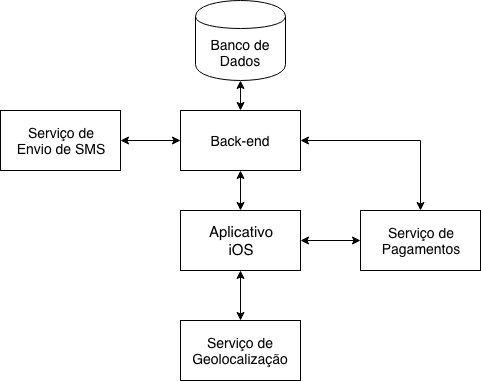
\includegraphics[width=0.8\textwidth]{pfc/figuras/system-architecture.png}
    \caption{Arquitetura global dos sistemas envolvidos}
    \label{fig:architecture}
\end{figure}
